\chapter{Bayesian Statistics}
\label{cap:bayes}

\emph{Bayesian statistics} is a particular approach to applying probability to statistical problems. It provides us with mathematical tools to update our beliefs about random events in light of seeing new data or evidence about those events.

In particular Bayesian inference interprets probability as a measure of confidence that an individual may possess about the occurrence of a particular event.

We may have a \emph{prior belief} about an event, but our beliefs are likely to change when \emph{new evidence} is brought to light. Bayesian statistics gives us a solid mathematical means of incorporating our prior beliefs, and evidence, to produce \emph{new posterior beliefs}.

This is in contrast to another form of statistical inference, known as \emph{frequentist statistics}, which assumes that probabilities are the frequency of particular random events occurring in a long run of repeated trials.

For example, as we roll a fair six-sided die repeatedly, we would see that each number on the die tends to come up 1/6 of the time.

\section{Frequentist vs Bayesian}
When carrying out statistical inference, that is, inferring statistical information from probabilistic systems, the two approaches, frequentist and Bayesian, have very different philosophies.

Frequentist statistics tries to eliminate uncertainty by providing estimates. Bayesian statistics tries to preserve and refine uncertainty by adjusting individual beliefs in light of new evidence.

In order to make clear the distinction between the two differing statistical philosophies, we will consider two examples of probabilistic systems:
\begin{itemize}
\item Coin flips, what is the probability of an unfair coin coming up head ?
\begin{itemize}
	\item \textbf{frequentist}: the probability of seeing a head when the unfair coin is flipped is the long-run relative frequency of seeing a head when repeated flips of the coin are carried out. That is, as we carry out more coin flips the number of heads obtained as a proportion of the total flips tends to the "true" probability of the coin coming up as head. In particular the individual running the experiment does not incorporate her own beliefs about the fairness of the coin.
	\item \textbf{Bayesian}: prior to any flip of the coin an individual may believe that the coin is fair. After a few flips the coin continually comes up head. Thus the prior belief about fairness of the coin is modified to account for the fact that three heads have come up in a row and thus the coin might not be fair. After 500 flips, with 400 heads, the individual believes that the coin is very unlikely to be fair. The posterior belief is heavily modified from the prior belief of a fair coin.
\end{itemize}
\item Election of a particular candidate for UK Prime Minister, what is the probability of seeing an individual candidate winning, who has not stood before ? (i.e. the candidate only ever stands once for this particular election and so we cannot perform "repeated trials") 
\begin{itemize}
	\item \textbf{frequentist}: here we construct "virtual" trials of the election process. The probability of the candidate winning is defined as the relative frequency of the candidate winning in the "virtual" trials as a fraction of all trials.	
	\item \textbf{Bayesian}: an individual has a prior belief of a candidate's chances of winning an election and their confidence can be quantified as a probability. However another individual could also have a separate differing prior belief about the same candidate's chances. As new data arrives, both beliefs are (rationally) updated by the Bayesian procedure.
\end{itemize}
\end{itemize}

Thus in the Bayesian interpretation a probability is a summary of an individual's opinion. A key point is that different (intelligent) individuals can have different opinions (and thus different prior beliefs), since they have differing access to data and ways of interpreting it. However, as both of these individuals come across new data that they both have access to their (potentially differing) prior beliefs will lead to posterior beliefs that will begin converging towards each other under the rational updating procedure of Bayesian inference.

In the Bayesian framework an individual would apply a probability of 0 when there is no confidence in an event occurring, while he would apply a probability of 1 when he is absolutely certain of an event occurring. A probability assigned between 0 and 1 allows weighted confidence in other potential outcomes.

In order to carry out Bayesian inference, we need to utilize a famous theorem in probability known as \emph{Bayes' rule} and interpret it in the correct fashion.

\section{Conditional Probability}
\label{sec:conditional_prob}
We begin by considering the definition of \emph{conditional probability}, which gives us a rule for determining the probability of an event $A$, given the occurrence of another event $B$. For example "what is the probability of rain occurring given that there are clouds in the sky ?"
To derive the general formula let's start with an example.

A fair die is rolled. Let $A$ be the event set that the outcome is an odd number ($A={1,3,5}$). Also let $B$ be the event set that the outcome is less than or equal to $3$ ($B={1,2,3}$). What is the probability of $A$ ($P(A)$) ? And what is the probability of $A$ given $B$, the probability we get $A$ conditioned to having also $B$ and denoted with $P(A|B)$ ?

Being a simple example we can compute the result by hand:

\begin{equation}
P(A) = \cfrac{|A|}{|S|} = \cfrac{|\{1,3,5\}|}{6} = \cfrac{1}{2}\qquad\textrm{(where S is the entire sample space)}
\end{equation}

Now let's find the conditional probability of $A$ given that $B$ occurred. If we know $B$ has occurred, the outcome must be among $\{1,2,3\}$. For $A$ to also happen the outcome must be in $A\cap B = \{1,3\}$. Since all die rolls are equally likely, we argue that $P(A|B)$ must be equal to

\begin{equation}
P(A|B) = \cfrac{|A\cap B|}{|B|} = \cfrac{2}{3}
\end{equation}

To find the mathematical definition we can rewrite the calculation by dividing the numerator and denominator by the entire space of the events $|S|$ hence:

\begin{equation}
  P(A|B) = \cfrac{|A\cap B|}{|B|} = \cfrac{\cfrac{|A\cap B|}{|S|}}{\cfrac{|B|}{|S|}} = \cfrac{P(A\cap B)}{P(B)}
  \label{eq:conditional_prob}
\end{equation}

This simply states that the probability of $A$ occurring given that $B$ has occurred is equal to the probability that they have both occurred, relative to the probability that $B$ has occurred.
Or in the language of the example above: the probability of rain given that we have seen clouds is equal to the probability of rain and clouds occurring together, relative to the probability of seeing clouds at all.
See Figure~\ref{fig:conditional_prob} for a graphical interpretation of conditional probability.

\begin{figure}[tb]
  \centering
  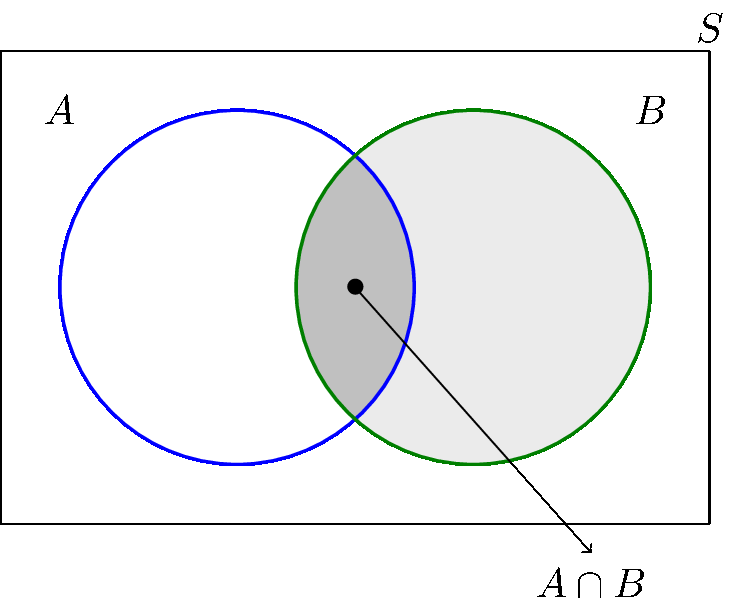
\includegraphics[width=0.5\linewidth]{figures/conditional_b}
  \caption{Graphical representation of conditional probability (the gray shaded area).}
  \label{fig:conditional_prob}
\end{figure}

\section{Bayes' Rule}

If we multiply both sides of Eq.~\ref{eq:conditional_prob} by $P(B)$ we get:
\begin{equation}
P(B)P(A|B)=P(A\cap B)
\end{equation}

But, we can simply make the same statement about $P(B|A)$, which is akin to asking "what is the probability of seeing clouds, given that it is raining?":

\begin{equation}
  P(B|A)=\frac{P(B\cap A)}{P(A)}
\end{equation}
Note that $P(A\cap B) = P(B\cap A)$ (i.e. having together events $A$ and $B$ is the same as having together events $B$ and $A$) and so by substituting the above and multiplying by $P(A)$, we get:
\begin{equation}
  P(A)P(B|A)=P(A\cap B)
\end{equation}

We are now able to set the two expressions for $P(A\cap B)$ equal to each other:
\begin{equation}
  P(A)P(B|A)=P(B)P(A|B)
\end{equation}
If we now divide both sides by $P(B)$ we arrive at the celebrated Bayes' rule:
\begin{equation}
  P(A|B)=\frac{P(B|A)P(A)}{P(B)}
\end{equation}

However, it will be helpful for later usage to modify the denominator, $P(B)$ on the right hand side to be written in terms of $P(B|A)$. From the \emph{law of total probability} we can actually write:
\begin{equation}
P(B)=\sum_{a\in A}P(B\cap a)
\end{equation}
this is possible if the events $A$ are an exhaustive partition of the sample space. So that by substituting the definition of conditional probability we get:
\begin{equation}
P(B)=\sum_{a\in A}P(B\cap a) = \sum_{a\in A}P(B|a)P(a)  
\end{equation}

Finally, we can substitute this into Bayes' rule from above to obtain an alternative version, which is used heavily in Bayesian inference:
\begin{equation}
P(A|B)=\frac{P(B|A)P(A)}{\sum_{a\in A}P(B|A)P(A)}
\end{equation}

\section{Applying Bayes' Rule for Bayesian Inference}
The basic idea of Bayesian inference is to continually update our prior beliefs about events as new evidence is presented. This is a very natural way to think about probabilistic events. As more and more evidence is accumulated our prior beliefs are steadily "washed out" by any new data.

Consider a (rather nonsensical) prior belief that the Moon is going to collide with the Earth. For every night that passes, the application of Bayesian inference will tend to correct our prior belief to a posterior belief that the Moon is less and less likely to collide with the Earth, since it remains in orbit.

In order to demonstrate a concrete numerical example of Bayesian inference it is necessary to introduce some new notation.

Firstly, we need to consider the concept of \emph{parameters} and \emph{models}. A \emph{parameter} could be the weighting of an unfair coin, which we could label as $\theta$. Thus $\theta = P(H)$ would describe the probability distribution of our beliefs that the coin will come up as head ($H$) when flipped. The \emph{model} is the actual means of encoding this flip mathematically. In this instance, the coin flip can be modeled as a \emph{Bernoulli trial}. A Bernoulli trial is a random variable with only two outcomes, usually labeled as "success" or "failure", in which the probability of the success is exactly the same every time the trial is carried out. The probability of the success is given by $\theta$, which is a number between 0 and 1. Thus $\theta\in[0,1]$.

Over the course of carrying out some coin flip experiments (repeated Bernoulli trials) we will generate some data, $D$, about heads or tails. A natural question to ask is "what is the probability of seeing 3 heads in 8 flips (8 Bernoulli trials), given a fair coin ($\theta=0.5$) ?".

%A model helps us to ascertain the probability of seeing this data, $D$, given a value of the parameter $\theta$.
The probability of seeing data $D$ under a particular value of $\theta$ is given by $P(D|\theta)$. However, if you consider it for a moment, we are actually interested in the alternative question, "what is the probability that the coin is fair (or unfair), given that I have seen a particular sequence of heads and tails ?".

Thus we are interested in the \emph{probability distribution} which reflects our belief about different possible values of $\theta$, given that we have observed some data $D$, denoted by $P(\theta|D)$. Notice that this is the converse of $P(D|\theta)$. The Bayes' rule is the link that allows us to go between the two situations.
\begin{equation}
  P(\theta|D) = P(D|\theta)P(\theta)/P(D)
\end{equation}
where:
\begin{itemize}
\item $P(\theta)$ is the \emph{prior}. This is the strength in our belief of $\theta$ without considering the evidence. Our prior view on the probability of how fair the coin is.
\item $P(\theta|D)$ is the \emph{posterior}. This is the (refined) strength of our belief of $\theta$ once the evidence $D$ has been taken into account. After seeing 4 heads out of 8 flips, say, this is our updated view on the fairness of the coin.
\item $P(D|\theta)$ is the \emph{likelihood}. This is the probability of seeing the data $D$ as generated by a model with parameter $\theta$. If we knew the coin was fair, this tells us the probability of seeing a number of heads in a particular number of flips.
\item $P(D)$ is the \emph{evidence}. This is the probability of the data as determined by summing (or integrating) across all possible values of $\theta$, weighted by how strongly we believe in those particular values of $\theta$. If we had multiple views of what the fairness of the coin is (but didn't know for sure), then this tells us the probability of seeing a certain sequence of flips for all possibilities of our belief in the coin's fairness.
\end{itemize}

The entire goal of Bayesian inference is to provide us with a rational and mathematically sound procedure for incorporating our prior beliefs, with any evidence at hand, in order to produce an updated posterior belief. What makes it such a valuable technique is that posterior beliefs can themselves be used as prior beliefs under the generation of new data. Hence Bayesian inference allows us to continually adjust our beliefs under new data by repeatedly applying Bayes' rule.

Note that in the derivation of the Bayes Theorem we have used the conditional probability definition. Indeed Bayes's formula actually connects two different conditional probabilities $P(A|B)$ and $P(B|A)$, and is essentially a formula for "turning the conditioning around". The Reverend Thomas Bayes referred to this in terms of "inverse probability".

Let's see now a concrete example using the age-old tool of statisticians: the coin-flip.

\subsection{Coin-Flipping Example}
Consider multiple flips of a coin with unknown fairness. We will use Bayesian inference to update our beliefs on the fairness of the coin as more data (i.e. more coin flips) becomes available. The coin will actually be fair, but we won't learn this until the trials are carried out. At the start we have no prior belief on the fairness of the coin, that is, we can say that any level of fairness is equally likely.

In statistical language we are going to perform $N$ repeated Bernoulli trials with $\theta=0.5$. %We will use a \emph{uniform distribution} as a means of characterising our prior belief that we are unsure about the fairness. This states that we consider each level of fairness (or each value of $\theta$) to be equally likely.
We are going to use a Bayesian updating procedure to go from our prior beliefs to posterior beliefs as we observe new coin flips. 
This process can be quite complicated in the general case but for this particular example the concept of \emph{conjugate priors} can be used.

\subsection{Conjugate Priors}
We have just outlined Bayes' rule and have seen that we must specify a likelihood function, a prior belief and the evidence (i.e. a normalizing constant). Let's take a closer look to the likelihood using again the coin-flips example.

We are interested in the probability of the coin coming up head as a function of the underlying fairness parameter $\theta$.
If we denote by $k$ the random variable that describes the result of the coin toss, which is drawn from the set $\{1, 0\}$, where $k=1$ represents a head and $k=0$ represents a tail, then the probability of seeing a head, with a particular fairness of the coin, is given by:
\begin{equation}
  P(k=1|\theta) = \theta 
\end{equation}
And the probability of coming up tail as:
\begin{equation}
  P(k=0|\theta) = 1-\theta 
\end{equation}
This can also be written as:
\begin{equation}
  P(k|\theta) = \theta^k(1-\theta)^{1-k} 
\end{equation}

This is known as the \emph{Bernoulli distribution}, in essence it tells us the probability of a coin coming up head or tail depending on how fair the coin is.

We can also consider another way of looking at the above function. If we consider a fixed observation, i.e. a known coin flip outcome, $k$, and the fairness parameter $\theta$ as a continuous variable then it tells us the probability of a fixed outcome $k$ given some particular value of $\theta$. As we adjust $\theta$ (e.g. change the fairness of the coin), we will start to see different probabilities for $k$.

This is known as the \emph{likelihood function} of $\theta$. Note that the likelihood function is not actually a probability distribution in the true sense since integrating it across all values of the fairness parameter $\theta$ does not actually equal 1, as is required for a probability distribution.

With the Bernoulli likelihood function we can determine the probability of seeing a particular sequence of flips, given by the set $\{k_1,\ldots,k_N\}$. Since each of these flips is independent of any other, the probability of the sequence occurring is simply the product of the probability of each flip occurring.

If we have a particular fairness parameter $\theta$, then the probability of seeing this particular stream of flips, given $\theta$, is given by:
\begin{equation}
  P(\{k\}|\theta)=\prod_{i}P(k_i|\theta)=\prod_i \theta^{k_i}(1-\theta)^{1-k_i}
\end{equation}

What about if we are interested in the number of heads, say, in $N$ flips? If we denote by $z$ the number of heads appearing, then the formula above becomes:
\begin{equation}
  P(z,N|\theta) = \binom{N}{z}\theta^z(1-\theta)^{N-z}
\end{equation}
where $\binom{N}{z}$ is the binomial coefficient. That is, the probability of seeing $z$ heads, in $N$ flips, assuming a fairness parameter $\theta$. 

\subsubsection{Quantifying our Prior Beliefs}
In the Bayesian approach we need to determine our prior beliefs on parameters and then find a probability distribution that quantifies these beliefs.
In this example we are interested in our prior beliefs on the fairness of the coin. That is, we wish to quantify our uncertainty in how biased the coin is. $\theta=0$ indicates a coin that always comes up tail, while $\theta=1$ implies a coin that always comes up head. A fair coin is denoted by $\theta=0.5$.

The question then becomes, which probability distribution do we use to quantify our beliefs about the coin ?

In this instance we are going to choose the \emph{beta distribution}. The probability density function of the beta distribution is given by:
\begin{equation}
	P(\theta|\alpha,\beta)=\theta^{\alpha -1}(1-\theta)^{\beta-1}/B(\alpha,\beta)
\end{equation}
where the term in the denominator, $B(\alpha,\beta)$ is present to act as a normalizing constant so that the area under the PDF actually sums to 1.

\begin{figure}[htb]
  \centering
  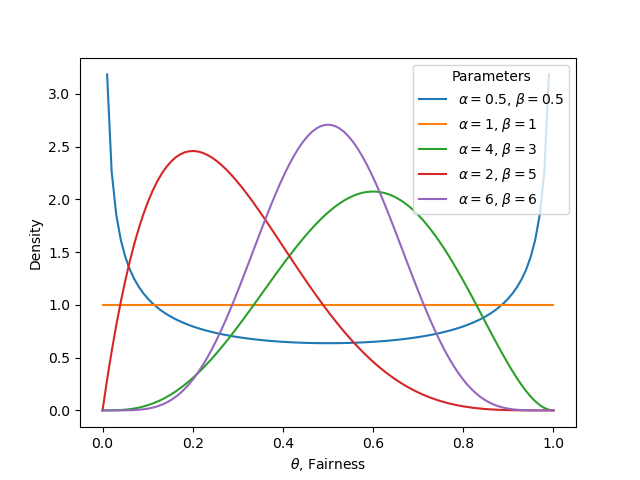
\includegraphics[width=.7\textwidth]{figures/beta_distro}
  \caption{Different realizations of the beta distribution for various parameters $\alpha$ and $\beta$.}
  \label{fig:beta_distro}
\end{figure}

Essentially, as $\alpha$ becomes larger the bulk of the probability distribution moves towards the right (a coin biased to come up heads more often), whereas an increase in $beta$ moves the distribution towards the left (a coin biased to come up tails more often).
However, if both parameters increase then the distribution begins to narrow. If they both increase equally, then the distribution will peak over $\theta=05$, i.e. when the coin is far. Note also that the \emph{uniform distribution} is a particular case of a beta distribution (i.e. $\alpha = \beta = 1$).

Among various interesting properties we have chosen the beta function as our prior because it is a conjugate prior for the Bernoulli distribution.

\subsubsection{Conjugate Prior}
In Bayes' rule we can see that the posterior distribution is proportional to the product of the prior distribution and the likelihood function:
\begin{equation}
  P(\theta|D)\propto P(D|\theta)P(\theta)
\end{equation}

A \emph{conjugate prior} is a choice of prior distribution, that when coupled with a specific type of likelihood function, provides a posterior distribution that is of the \emph{same family} as the prior distribution, i.e. the prior and posterior both have the same probability distribution family, but with differing parameters.

Conjugate priors are extremely convenient from a calculation point of view as they provide closed-form expressions for the posterior, thus negating any complex numerical integration.

In our case, if we use a Bernoulli likelihood function AND a beta distribution as the choice of our prior, we immediately know that the posterior will also be a beta distribution.

%Using a beta distribution for the prior in this manner means that we can carry out more experimental coin flips and straightforwardly refine our beliefs. The posterior will become the new prior and we can use Bayes' rule successively as new coin flips are generated.

We can actually use a simple calculation to prove why the choice of the beta distribution for the prior, with a Bernoulli likelihood, gives a beta distribution for the posterior.

As mentioned above, the probability density function of a beta distribution, for our particular parameter $\theta$, is given by:
\begin{equation}
  P(\theta|\alpha,\beta)=\theta^{\alpha -1}(1-\theta)^{\beta-1}/B(\alpha,\beta)
\end{equation}

You can see that the form of the beta distribution is similar to the form of a Bernoulli likelihood. In fact, if we multiply the two together, we get:
\begin{equation}
  \theta^{\alpha -1}(1-\theta)^{\beta-1}/B(\alpha,\beta)\times \theta^k(1-\theta)^{1-k} \propto \theta^{\alpha+k-1}(1-\theta)^{\beta+k}
\end{equation}

Notice that the term on the right hand side of the proportionality sign has the same form as our prior (up to a normalizing constant).

The last issue we need to address is how to connect $\alpha$ and $\beta$ parameters to more intuitive parameters like mean and variance. It turns out that we can use the following relationships:
\begin{equation}
  \begin{gathered}
    \mu = \frac{\alpha}{\alpha+\beta} \\
    \sigma = \sqrt{\frac{\alpha\beta}{(\alpha + \beta)^2(\alpha + \beta + 1)}}
  \end{gathered}
\end{equation}

Re-arrange these formulae 
\begin{equation}
  \begin{gathered}
    \alpha = \left(\frac{1-\mu}{\sigma^2} - \frac{1}{\mu} \right) \mu^2\\
    \beta = \alpha\left(\frac{1}{\mu}-1 \right)
  \end{gathered}
\end{equation}

%Note that we have to be careful here, as we should not specify a , since this is the standard deviation of a uniform density (which itself implies no prior belief on any particular fairness of the coin).

So suppose I think the fairness of the coin is around 0.5, but I'm not particularly certain, I may specify a standard deviation of about 0.1. Plugging in the numbers into the above formulae gives us $\alpha = 12$ and $\beta = 12$ and the beta distribution in this instance looks like the following:
\begin{figure}[htb]
  \centering
  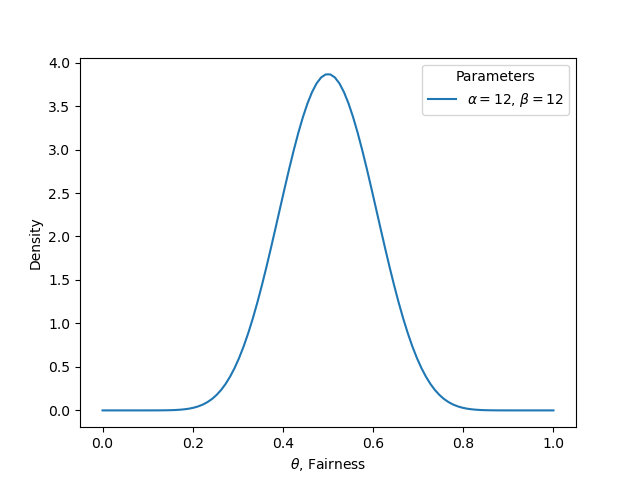
\includegraphics[width=.7\textwidth]{figures/beta_12_12}
  \caption{A beta distribution with $\alpha=12$ and $\beta=12$.}
  \label{fig:beta_12_12}
\end{figure}

Notice how the peak is centered around 0.5 but that there is significant uncertainty in this belief, represented by the width of the curve.

\subsection{Using Bayes' Rule to Calculate a Posterior}

We are now finally in a position to be able to calculate our posterior beliefs using Bayes' rule for repeated coin-flips
\begin{equation}
  P(\theta|z,N)=P(z,N|\theta)P(\theta)/P(z,N)
\end{equation}

If we substitute in the values for the likelihood function calculated above, as well as our prior belief beta distribution, we get:
\begin{equation}
  P(\theta|z,N)\propto P(z,N|\theta)P(\theta)\propto \theta^{z+\alpha - 1}(1-\theta)^{N-z+\beta -1} 
\end{equation}
so the posterior is given by $\textrm{beta}(\theta|z+\alpha,N-z+\beta)$ .
All we need do is specify the mean and standard deviation of our prior beliefs, carry out $N$ flips and observe the number of heads $z$ and we automatically have a rule for how our beliefs should be updated.

In Fig.~\ref{fig:bayes} we can see six particular points at which we have carried out a number of coin flips. In the top-left plot we have carried out no trials and our probability density function (in this case our original prior density) is the uniform distribution.
Originally we were not able to assume anything about the coin fairness, so the result states that we have equal belief in all values of $\theta$.

The next plot shows 2 trials carried out and they both come up heads. Our Bayesian procedure allows us to update to a posterior density. Notice how the weight of the density is now shifted to the right hand side of the chart. This indicates that our prior belief of equal likelihood of fairness of the coin, coupled with 2 new data points, leads us to believe that the coin is more likely to be unfair (biased towards heads than it is tails).

The following two plots show 10 and 20 trials respectively. Notice that since we have seen 6 tails in 10 trials we are now more convinced that the coin is likely to be unfair and biased towards tails. After 20 trials, we have seen a few more heads appear. The density of the probability has now shifted closer to $\theta = P(H) = 0.5$. Hence we are now starting to believe that the coin is possibly fair.

After 50 and 500 trials respectively, we are now beginning to believe that the fairness of the coin is very likely to be around $\theta=0.5$. This is indicated by the shrinking width of the probability density, which is now clustered tightly around $\theta=0.5$ in the final panel. Were we to carry out another 500 trials (since the coin is actually fair) we would see this probability density become even tighter and centered closer to $\theta=0.5$.

\begin{figure}[htb]
  \centering
  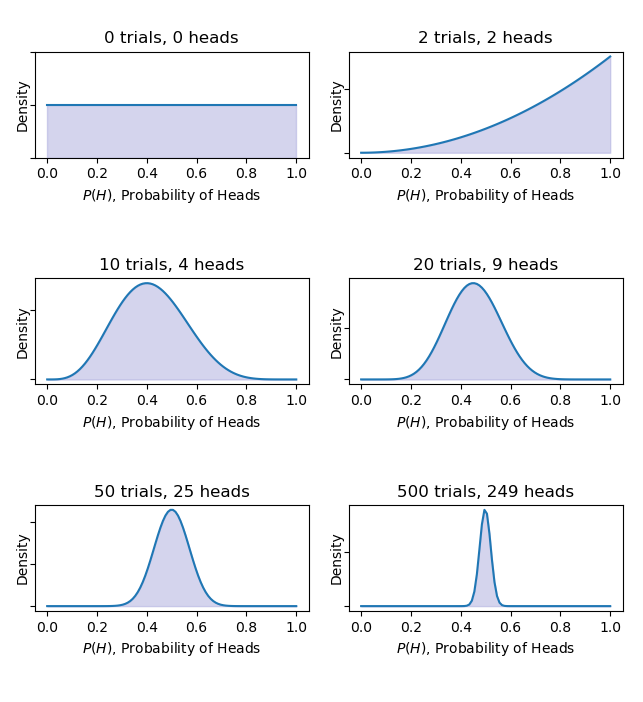
\includegraphics[width=.7\textwidth]{figures/bayes}
  \caption{Bayesian update procedure using the Beta-Binomial model.}
  \label{fig:bayes}
\end{figure}

Thus it can be seen that Bayesian inference gives us a rational procedure to go from an uncertain situation with limited information to a more certain situation with significant amounts of data.

\begin{finmarkets}
Below code implements the 
\end{finmarkets}

\begin{ipython}
import numpy as np
from scipy import stats
from matplotlib import pyplot as plt

number_of_trials = [0, 2, 10, 20, 50, 500]

data = stats.bernoulli.rvs(0.5, size=number_of_trials[-1])
x = np.linspace(0, 1, 100)

for i, N in enumerate(number_of_trials):
    heads = data[:N].sum()

    ax = plt.subplot(int(len(number_of_trials) / 2), 2, i + 1)
    ax.set_title("%s trials, %s heads" % (N, heads))
	
    plt.xlabel("$P(H)$, Probability of Heads")
    plt.ylabel("Density")
    if i == 0:
        plt.ylim([0.0, 2.0])
    plt.setp(ax.get_yticklabels(), visible=False)	
    y = stats.beta.pdf(x, 1 + heads, 1 + N - heads)
    plt.plot(x, y, label="observe %d tosses,\n %d heads" % (N, heads))
    plt.fill_between(x, 0, y, color="#aaaadd", alpha=0.5)
    
plt.tight_layout()
plt.show()
\end{ipython}

\section*{Exercises}
%\begin{question}
Using the function \texttt{randint} of the module \texttt{random} make a Monte Carlo simulation of rolling three dices to check the probability of getting the same values on the three of them.
From the probability theory you should expect:

\[P_{d1=d2=d3} = \frac{1}{6}\cdot\frac{1}{6}\cdot\frac{1}{6}\cdot 6 = \frac{1}{36} = 0.0278\]
\end{question}

\cprotEnv\begin{solution}
\begin{ipython}
from random import seed, randint

seed(1)
trials = 10000000
success = 0

for _ in range(trials):
    d1, d2, d3 = randint(1, 6), randint(1, 6), randint(1, 6)
    if d1 == d2 and d2 == d3:
        success += 1

print ("The probability to get three equal dice is {:.4f}".format(success/trials))

The probability to get three equal dice is 0.0278
\end{ipython}
\end{solution}

\begin{question}
Two fair dice are rolled, find the probability that their sum is:
\begin{enumerate}[start=1]
	\item equal to 1;
	\item equal to 4;
	\item less than 13.
\end{enumerate}
	
\noindent\textbf{Hint:} the possible combinations of the outcomes of two dice are 36 (to realize it you can simply think that for each one of the six faces of the first die you have six possible faces of the second hence $6\cdot 6=36$). It is not possible to get 1 since the dice have no face with 0 so the first probability should come out 0. The sum of the two dice is always less than 13 (the maximum is 12\ldots) so the answer to point 3 is 1. We can get a sum of 4 in 3 cases (1-3, 3-1 or 2-2) so the expected probability is $3/36=1/12=0.0833$
\end{question}

\cprotEnv\begin{solution}
\begin{ipython}
import random

random.seed(1)
successes = {"=1":0.0, "=4":0.0, "<13":0.0}
trials = 100000

for _ in range(trials):
    d1 = random.randint(1, 6)
    d2 = random.randint(1, 6)

    if (d1 + d2) == 1:
        successes["=0"] += 1.0
    if (d1 + d2) == 4:
        successes["=4"] += 1.0
    if (d1 + d2) < 13:
        successes["<13"] += 1.0

for k,v in successes.items():
    print ("P({}): {:.3f}".format(k, v/trials))

P(=1): 0.000
P(=4): 0.084
P(<13): 1.000
\end{ipython}
\end{solution}

\begin{question}
There are 60 chemical flasks in the laboratory, 6 of which are incorrectly labeled. What is the chance that if we randomly choose 5 flasks, exactly 3 of them will be labeled correctly ?

\noindent\textbf{Hint:} the probability is approximately 0.5 \%.
\end{question}

\cprotEnv\begin{solution}
\begin{ipython}
import random

flasks = ["C"]*54 + ["U"] * 6
random.seed(1)
trials = 1000
success = 0.

for _ in range(trials):
    draw = random.sample(flasks, 5)
    if draw.count("U") == 3:
        success += 1.

print ("Probability: {:.3f}%".format(success/float(trials)*100))

Probability: 0.499%
\end{ipython}
\end{solution}

\begin{question}
Given the following historical series (1895-2020) find average September temperature in US and report the 99\% confidence interval of your measure.
\noindent
Input (temperatures are in Fahrenheit degrees): \href{https://raw.githubusercontent.com/matteosan1/finance_course/develop/libro/input_files/histo_temp.csv}{histo\_temp.csv}
\end{question}

\cprotEnv\begin{solution}
\begin{ipython}
from scipy.stats import norm
import numpy as np
import pandas as pd

# first download the input file
df = pd.read.csv("histo_temp.csv")
temperatures = df['T'].to_array()
alpha = 0.99

A = norm.ppf((1 + alpha)/2)
m, se = np.mean(temperatures), np.std(temperatures)
h = A*se/np.sqrt(len(temperatures))

print ("Avg temperature in September (US): {:.1f}".format(m))
print ("{:.1f}% confidence interval: +- {}".format(alpha*100, h))
Avg temperature in September (US): 65.1
99% confidence interval: +- 0.3
\end{ipython}
\end{solution}

\begin{question}
Using the function \texttt{normal} of \texttt{numpy.random} simulate the price of a stock which evolves according to a log-normal stochastic process with a daily rate of return \(\mu=0.1\) and a volatility \(\sigma=0.15\) for 30 days.
Also plot the price. Try to play with \(\mu\) and \(\sigma\) to see how the plot changes.
\end{question}

\cprotEnv\begin{solution}
\begin{ipython}
from numpy.random import normal, seed
from matplotlib import pyplot as plt
import math

S = 100
mu = 0.1
sigma = 0.15
T = 1
seed(1)

historical_series = [S]
for i in range(30):
    S = S * math.exp((mu - 0.5 * sigma * sigma) * T +
        sigma * math.sqrt(T) * normal())
    historical_series.append(S)

plt.plot(range(31), historical_series)
plt.xlabel("days")
plt.ylabel("Price of stock X")
plt.show()
\end{ipython}

\begin{figure}[htbp]
\begin{center}
  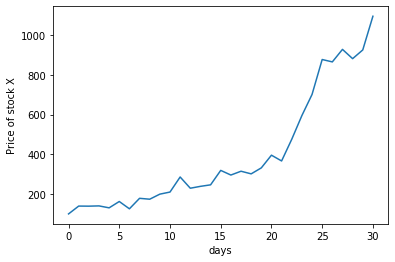
\includegraphics[width=0.7\linewidth]{figures/lesson6_solutions_5_0.png}
\end{center}
\end{figure}
\end{solution}


\begin{thebibliography}{9}
\bibitem{cit:bernoulli_distribution}\href{https://en.wikipedia.org/wiki/Bernoulli_distribution}{\emph{Bernoulli Distribution Wikipedia}}
\end{thebibliography}









